\subsection{Расстояние и размеры}
\textit{Годичный параллакс} --- это угол, под которым видно орбиту Земли с какой-либо звезды.
\begin{equation}r=\frac{1}{\pi}
\end{equation}
Где $r$ --- расстояние до звезды (в парсеках), $\pi$ --- годичный параллакс звезды (в секундах).
\begin{figure}[!h]
\centering
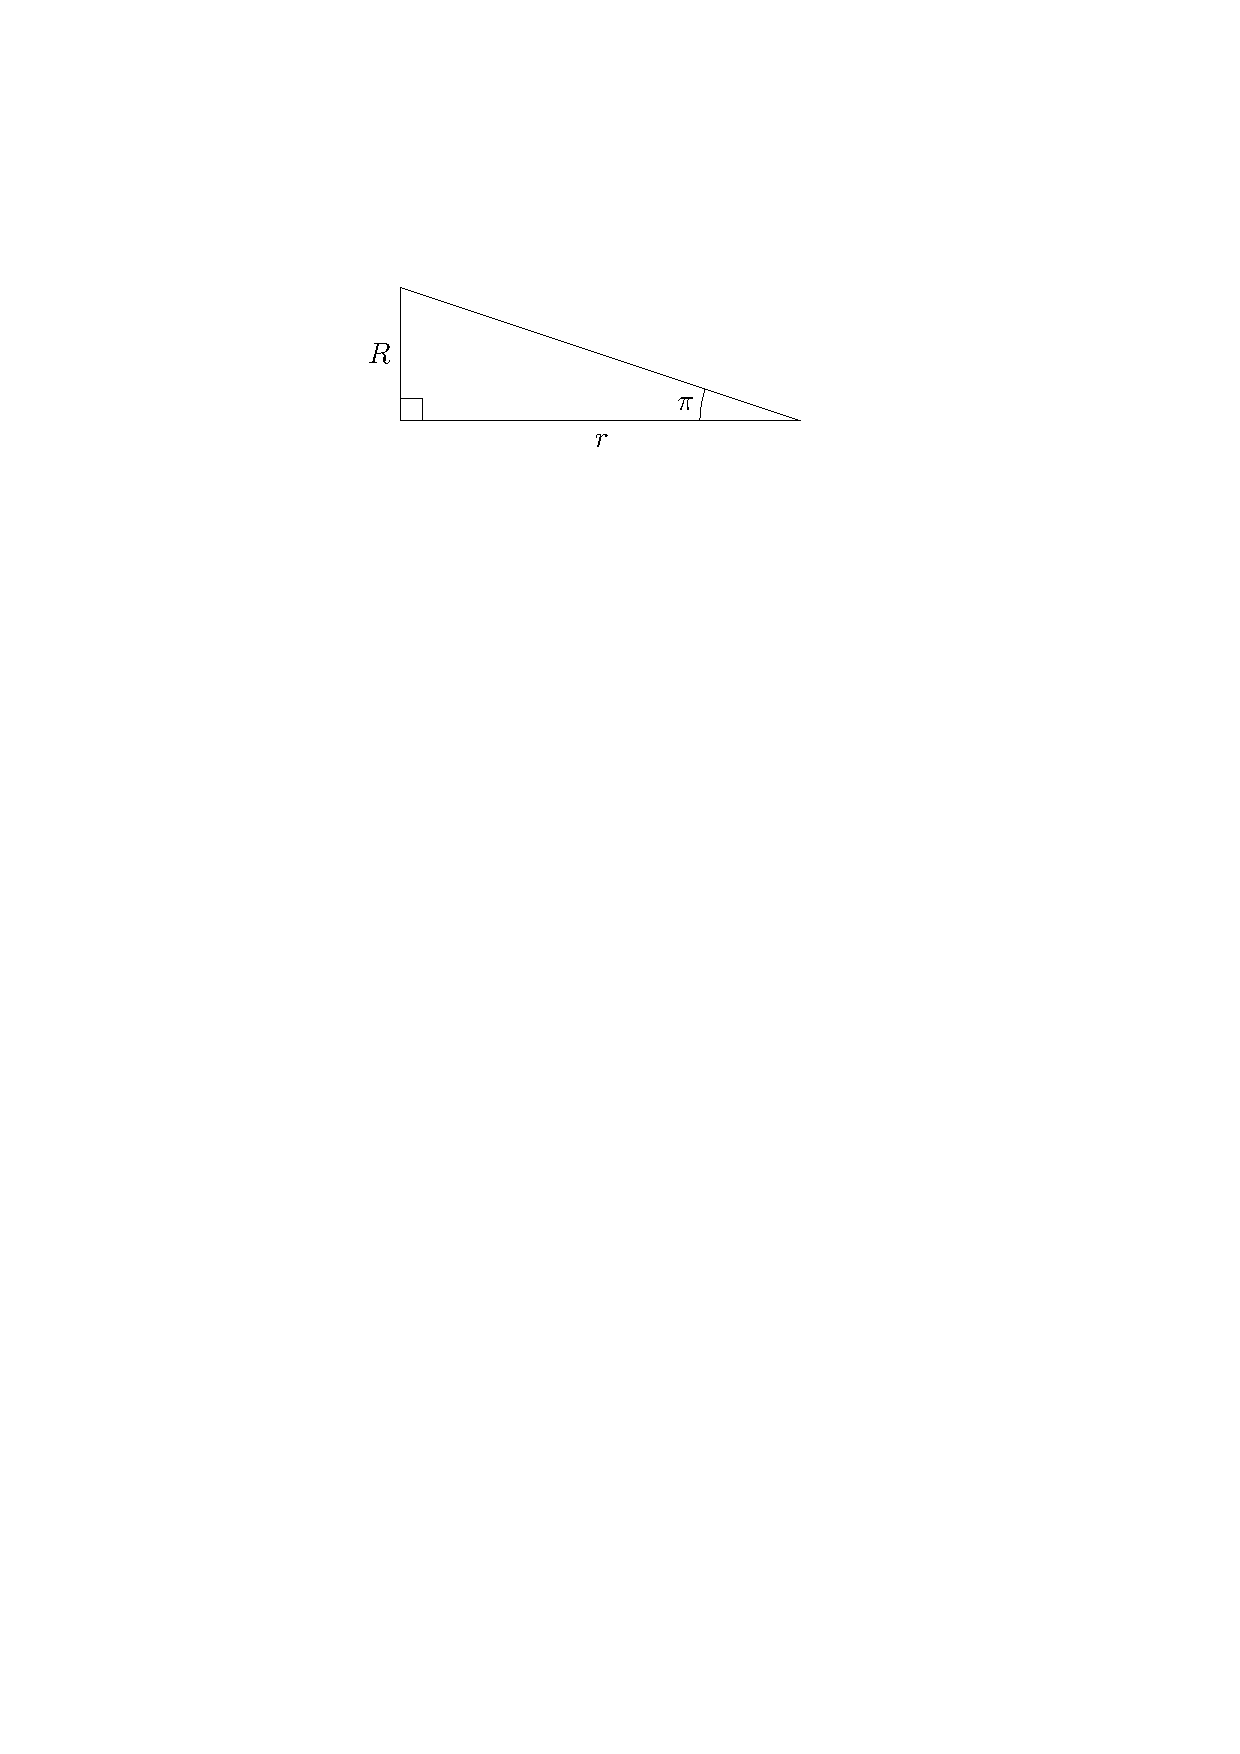
\includegraphics[width = 0.37\textwidth]{1-second}
\caption{Параллакс в одну секунду}
\end{figure}

Если $R$ --- радиус орбиты Земли, $r$ --- расстояние до объекта, $\pi$ --- годовой параллакс, то параллакс будет равен $\pi=1''$ с расстояния $r=1$пк.

В общем случае: 
\begin{equation}
\sin\pi=R/r
\end{equation}

Где $R$ и $r$ имеют одинаковые еденицы измернеий, но так как в одном парсеке 206265 а.е. и в одном радиане 206265 секунд, то,записывая радиус орбиты Земли в а.е., а расстояние звезды в парсеках, параллакс получается в секундах. Также, можно изменить $\sin\pi$ на $\pi$, потому что угол $\pi$ является малым углом. Таким образом, получается следующая формула:\begin{equation}
r_{\text{пк}}=\frac{1\text{ а.е.}}{\pi_{\text{сек}}}
\end{equation}


\textit{Горизонтальный параллакс} --- это угол, под которым видно радиус Земли, при положении светила на горизонте.
\begin{equation}r=\frac{R_{\text{З}}}{\sin p_0}=\frac{3438'}{p_0'}R_{\text{З}}=\frac{206265''}{p_0''}R_{\text{З}}
\end{equation}
Где $R_{\text{З}}$ --- радиус Земли, $p_0$ --- горизонтальный экваториальный параллакс.

\textbf{Правило Тициуса-Боде} --- эмпирическая формула приблизительно описывающая радиусы орбит планет от Солнца:
\begin{equation}r=\frac{3\cdot 2^n+4}{10}
\end{equation}
Где $n=-\infty, 0, 1, 2...$

\textit{Угловой размер объекта} --- это угол, под которым видно радиус объекта с Земли.
\begin{equation}\rho=\frac{R}{r}
\end{equation}
Где $R$ --- радиус объекта, $\rho$ --- угловые размеры объекта, $r$ --- растояние до объекта. Здесь также можно использовать приближение для малых углов: $\sin\rho\approx\rho$